\documentclass[a4paper, twocolumn, superscriptaddress, longbibliography]{revtex4-2}
\usepackage[colorlinks,urlcolor=blue,linkcolor=blue]{hyperref}
\usepackage[utf8]{inputenc}
\usepackage{graphicx}
\usepackage{geometry}
\usepackage{amsmath}
\usepackage{amssymb}
\usepackage{amsfonts}
\usepackage{hyperref}
\usepackage{dsfont}
\usepackage[dvipsnames]{xcolor}
\usepackage{appendix}

\hypersetup{citecolor=cyan}
\geometry{hmargin=2cm,vmargin=2cm}

\begin{document}
	\author{Maxime Debertolis}
	%\email{maxime.debertolis@uni-bonn.de}
	\affiliation{Institute of Physics, University of Bonn, Nu\ss allee 12, 53115 Bonn, Germany}
	\title{Gaussian augmented Tensor Networks for universal quantum simulations}

	\begin{abstract}

	\end{abstract}

	\maketitle

	\section{Introduction}
	
	Ansatz mixing a basis of orbitals to an MPS:
	\begin{equation}
		|\psi \rangle = \sum_{i=1}^{2^{L}} \nu_i^{} d_{\vec{b}_i}^{} |\psi_{\mathrm{G}}^{}\rangle,
	\end{equation}
	\emph{Gaussian states}:
	Majorana operators and fermionic operators are related as:
	\begin{equation}
		\hat{\gamma}_{2j-1} = c^{\dagger}_{j} + c_{j}, \;\;
		\hat{\gamma}_{2j} = -i ( c^{\dagger}_{j} + c_{j}),
	\end{equation}
	Covariance matrix: 
	\begin{equation}
		\Gamma_{ab}^{} = \frac{i}{2} \mathrm{Tr}\left(\rho[\gamma_a^{},\gamma_b^{}] \right)
	\end{equation}
	Gaussian state defined through fermionic operators:
	\begin{equation}
		\begin{split}
			|\psi_{\mathrm{G}}\rangle &= \prod_{j=1}^{L}\left(c_{j}^{\dagger}\right)^{n_j}|0\rangle, \\
			\rho_{\mathrm{G}}^{} &= \frac{1}{2^{L}}\prod\limits_{j=1}^{2L}\left(\mathds{1} + i\lambda_{j} \tilde{\gamma}_{2j-1}^{} \tilde{\gamma}_{2j}^{} \right)
		\end{split}
	\end{equation}
	This is valid in a given basis, where $n_j=\langle c^{\dagger}_j c^{}_j\rangle$ should also be known by diagonalizing the correlation or covariance matrix. We also have a	set of destabilizers formed by the set of odd majorana modes:
	\begin{equation}
	d^{}_i = \prod_{j=1}^{L}\tilde{\gamma}_{2j-1}^{\vec{b}_{i}(j)},
	\end{equation}
	in which $\vec{b}_i$ is a vector into which the binary representation of $i$ is encoded, such that $\vec{b}_{i}(j) \in \{0,1\}$ tells if the occupation of the orbital $j$ in the state to which the product of \emph{destabilizers} is applied will change. The set of state generated by the combination of the Gaussian state and the destabilizers form an orthonormal basis of Gaussian states for the Hilbert space of dimension $2^{L}$, since there are $2^L$ combination of the destabilizers, $d_j |\psi_{\mathrm{G}}\rangle$ is also a Gaussian state and $\langle \psi_{\mathrm{G}}^{}|d_i d_j |\psi_{\mathrm{G}}\rangle = \delta_{ij}$.
	
	The basis of majoranas evolves after each (local or global) Gaussian operations:
	\begin{equation}
		\tilde{\gamma}_j = \sum_{k=1}^{2L} R_{jk}\gamma_{k}
	\end{equation}
	The basis of natural orbitals can always be reconstructed through the rotated majoranas:
	\begin{equation}
		\tilde{c}_{j}^{} = \frac{1}{2}\left(\tilde{\gamma}_{2j-1} + i\,\tilde{\gamma}_{2j}\right),
	\end{equation}
	which form a set of \emph{stabilizers} that allows with the corresponding natural occupations to fully determine a Gaussian state.

	\emph{Algorithm}: Equipped with the GaMPS representation of the state that allows to span the entire Hilbert space, we present below how to apply a quantum circuit to the GaMPS.
	\begin{itemize}
		\item {\bf Gaussian operations}: Applying a Gaussian unitary $U_{\mathrm{G}}$ to the state is equivalent to update the basis of orbitals as $\tilde{\gamma}_j = \sum_{k=1}^{2L} G_{jk}\gamma_{k}$, as illustrated in Fig.~\ref{fig:sketch}. After each Gaussian operation, we update the orbital frame by successively multiplying the corresponding orthogonal transformations, thereby keeping track of the basis at all times. We dub this basis the instantaneous orbital basis, which defines the space spanned by physical legs in the associated MPS.
		\item {\bf Non-Gaussian operations}: The set of odd Majoranas (our \emph{destabilizers}) together with the even ones  forms a complete operator basis, allowing any operator to be expressed as $U = \sum_{i} \phi_{i} s_{u_i}d_{v_i}$. For a local gate acting on nearest neighbors, this representation corresponds to a local operation on the MPS. This decomposition remains particularly simple for the class of circuits illustrated in Fig.~\ref{fig:sketch}, where we consider the sequential application of Gaussian and non-Gaussian gates. However, if a non-Gaussian operation is only local in a basis differing from the instantaneous one, the corresponding gate to be applied on the MPS becomes highly nonlocal, potentially leading to an unbounded growth of entanglement.
		\item {\bf Expectation values}: Expectation values are evaluated by decomposing the observable in the instantaneous orbital basis, $\langle \psi | \hat{O} | \psi \rangle = \sum_{k=1}^{L^{r}} a_{k}\langle \nu | \hat{O}_k | \nu \rangle$, where $a_k$ denotes the weight associated with the operator $\hat{O}_{k}$ and $r$ is the number of fermionic modes encoded in the observable. For instance, a density operator $n_\alpha$ can be expanded as $n_\alpha = \sum_{ij} R^{*}_{i\alpha} R_{\alpha j} \hat{\tilde{c}}^{\dagger}_{i}\hat{\tilde{c}}^{}_{j}$, so that $a_{ij} = R^{*}_{i\alpha} R_{\alpha j}$.
	\end{itemize}

	\begin{figure*}[t]
		\centering
		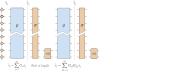
\includegraphics[width=1.\textwidth]{Figs/Sketch/Sketch_circuit.pdf}
		\caption{Sketch.}
		\label{fig:sketch}
	\end{figure*}

	\section{Conclusion and outlook}

	%\textit{Acknowledgement}. The author thank Neil Dowling and Julien Bréhier for discussions. The author was supported by the Deutsche Forschungsgemeinschaft through the cluster of excellence ML4Q (EXC 2004, project-id 390534769) and by the Deutsche Forschungs- gemeinschaft through CRC 1639 NuMeriQS (project-id 511713970).

	\bibliography{Biblio.bib}

      \begin{appendices}
	\end{appendices}


\end{document}

